\documentclass[12pt]{article}
\usepackage{graphicx}
\usepackage{times}
\usepackage{cite}
\usepackage[utf8]{inputenc}
\usepackage{subfig}
\usepackage{caption}
%this is a comment
\title{The Memo}
\author{Jesse Chick\\
\and Benjamin Martin\\
\and Keenan Johnson\\
\and Nickoli Londura\\
\and Jiaji Sun}




\begin{document}
\maketitle
\tableofcontents

\section{Contributors and ONIDs}
\par
LINK TO THE GITHUB REPO AT THE CORRECT BRANCH: https://github.com/Tonyenike/CS361-001-W2018/tree/the_memo-assignment-4/projects/martinb3/assignment-4

\begin{itemize}
	\item Jesse Chick $\sim$ chickj
	\item Benjamin Martin $\sim$ martinb3
	\item Keenan Johnson $\sim$ johnsoke
	\item Nickoli Londura $\sim$ londuran
	\item Jiaji Sun $\sim$ sunji
\end{itemize}

\section{UML Class Diagram}
	
	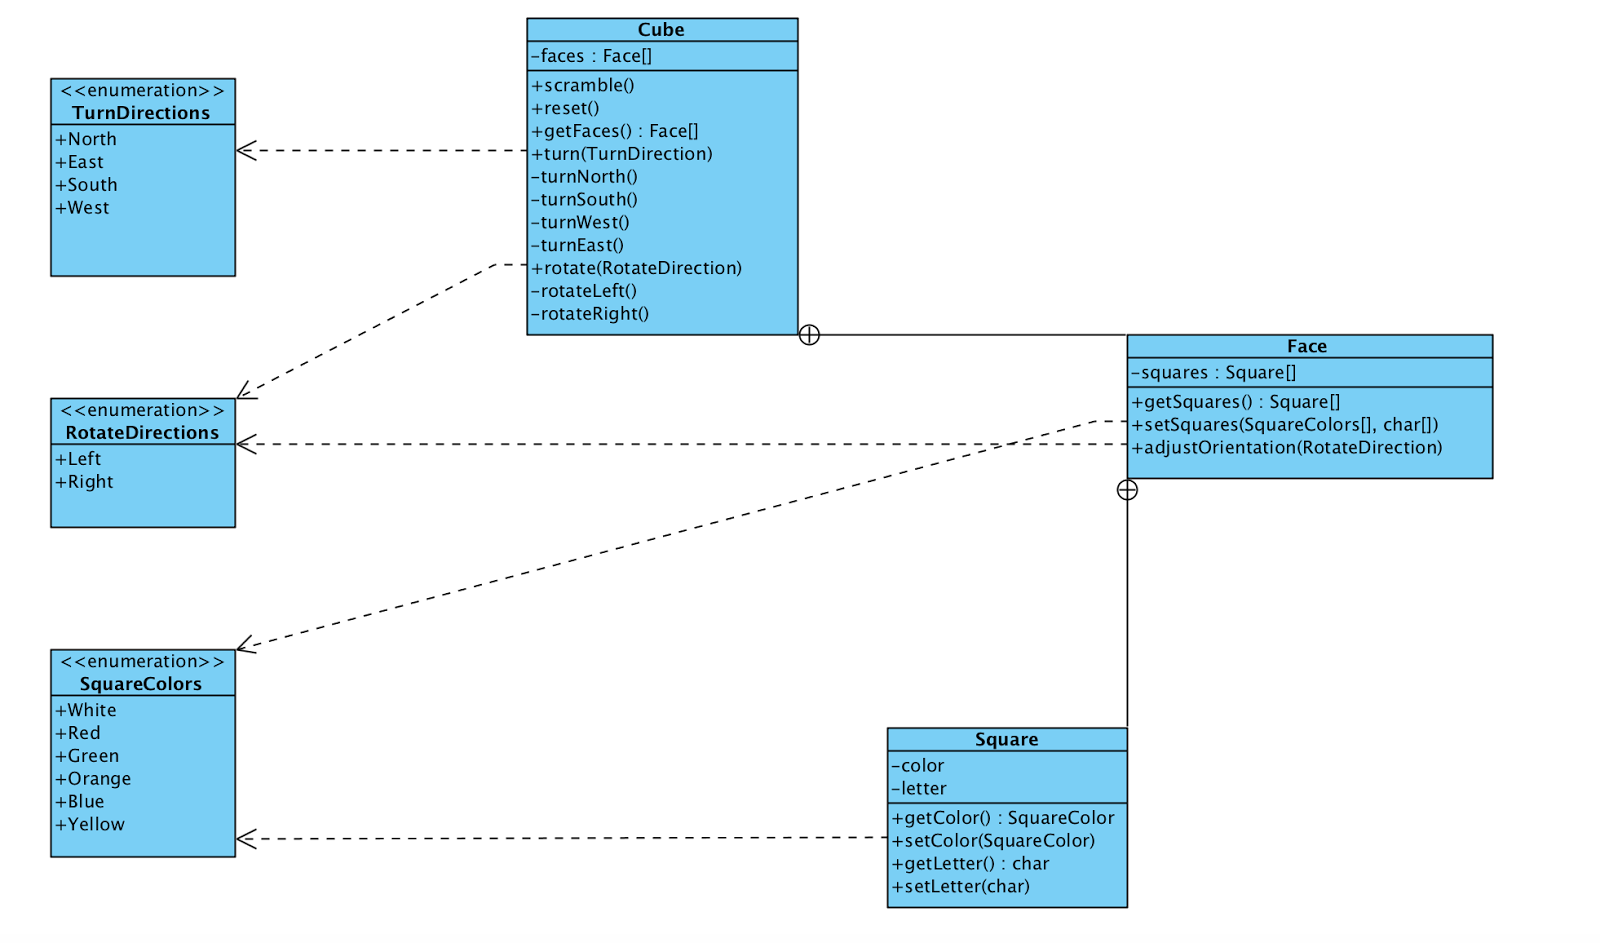
\includegraphics[width = \textwidth]{diagram.PNG}

\section{Packages}

\par
The main object of our project, the cube, is the most complex  in our application. This is where the most packaging can be seen as we are separating out each module to be as specific and focused as possible. We have the main “Cube” module that ties in and utilizes each other module. The rest are smaller modules focusing on single tasks related to the cube object overall. The “TurnDirections” module takes care of making turns and the “RotateDirections” takes care of rotating the cube object. Then we have the “Square” module that makes use of the “SquareColors” module to get the colors of each piece on the cube. Finally, the “Face” module compiles the square modules to generate one ‘face’ of the cube for the “Cube” module. In this cube object, cohesion is quite high. We broke down every function of the object and are creating an individual module for each. Coupling is also fairly high. The “Cube” module itself is completely reliant on each other function. The “Square” and “SquareColors” modules are tightly coupled together and also with the “Faces” module. \\

\par
For the rest of the application cohesion is pretty high as we only have a few more modules and each is already very specific to the tasks they perform (scramble generation, solution generation). Coupling is moderately high as the scrambles and solutions of the cube go hand in hand. We don’t want to produce mismatching solutions that don’t solve the scramble we provide. \\

\section{Design Patterns}
\par
When we designed the project, we want to create objects for our system. Each object will serve a purpose. The cube object contains six face objects, and the face object contains nine square objects (all of which could be named UR, UM, UL, etc) so that we have all of the information of the cube. This can also be used to manipulate the cube, which is easy to understand. The cube object will have the most functionality because it is the biggest component of the three different objects. There is no inheritance or polymorphism. We have only object containers. A face is not a subset or a child of a cube, and neither is a square a subset or a child of a face, so we have no inheritance or polymorphism in our program. For that reason, we opted to design using the structural patterns (SP) to implement our program. We also are using the behavioral patterns (BP) to display each page of our website. By creating each page of our website individually, we can show the behavioral pattern of each page, which is easy to understand and divide in the human mind. By separating our design patterns into these two categories, it is easy to tackle and accomplish the project: Each behavioral pattern has an associated structural pattern with its own associated objects/classes. Since each webpage is unique, each page requires its own functionality and objects; we cannot share objects across pages (unless merely for CSS design purposes). \\

\section{Exceptions and Handling}

\par
When working with systems, there could be many exceptions that could occur during implementation. When working with HTML, there could be many exceptions that can come up. If links are not working properly then the users will have a hard time with it. When this occurs, the exception could be handled by having an error message come up, explaining the cause of the problem, and automatically sending an error code to the developers. There could also be errors that come up when using a program on a webpage. When the user interacts with the tools provided to work the program, there could be an exception where they don’t function properly. These kinds of exceptions can be handled by having an option on the web page to send an error message to the the developers in order for the issues to be resolved. Looking more into the design of the system, exceptions can happen there as well. A possible exception could be that the parent class could have a function written incorrectly and that makes the child classes have problems. This could be handled by having the child class recognize the error and trace it back to the parent class, which then provides a specific error message. Another exception that's possible is having the parent class provide a connection to the wrong child class for one of the functions. This could be handled by having the user report an error to the developers in order for it to be fixed. Missing a class could also be an exception because each class a certain purpose for the program to work, and without one will cause errors. This can be handled by displaying an error message specifically for not having a certain class. All exceptions that could happen should be handled a certain way in order for future errors not to occur. \\

\section{Meeting Report}
\par
On this week we have met four times on campus. Including three times in library and one meeting after class. \\

\par
On our first meeting on Wednesday. We met everyone still in the library. we separate our third phase of the project to every group member. Jesse Chick is working on class diagrams and prepare for the presentation. Benjamin Martin is working on design patterns. Keenan Johnson is working on packages. He is preparing presentation also. Nickoli Londura is working on exceptions and handling. Jiaji Sun is working on meeting report. On this meeting, we have tried four different architectures. However, we found our first version architecture is much better than other solution. It’s the best solution for this project. The running time is shortest one and it is the easiest one to maintain. On the end of this meeting, we basically settle down our final version of UML class diagram. We decided to work on packages and design patterns for next meeting. \\

\par
On our second meeting on Thursday. We met everyone at the library again. We discussed how many packages and which packages do we need on our project. We have researched some packages from online. Base on our project situation, we decide to use three packages. After we settle down our packages. We started to work on design patterns. We have discussed many different design patterns for our project. However, there only two design patterns were fit our project. Therefore, we decided to choose those two design pattern to be our design pattern for our project. We decide to use structural patterns and behavioral patterns for our project. After we have done with packages and design patterns. We decided to work on exceptions and handling for next meeting. \\

\par
On our third meeting on Thursday. We met everyone again after class. We have a short conversation for plan our last meeting. After a brief discussed, we decided to make the last meeting on Saturday for working on exceptions and handling. \\

\par
On our last meeting on Saturday. We met everyone at the library again. We made some brainstorm for exceptions and handling first. We have to try to think every exceptions and handling as much as possible for that. Finally, we found two exceptions and handling for our project. \\


\cite{rubtut}

\bibliography{myref}
\bibliographystyle{plain}

\end{document}
